




IRS 63 is a Class I protostar embedded in the L1709 region of the Ophiuchus molecular cloud at a distance of 144 pc \citep{sadavoy_dust_2019, Dom2020}. It is one of the brightest Class I protostars at (sub)millimetre wavelengths, and is surrounded by a relatively large circumstellar disk with a radius larger than 50 AU \citep{Dom2020}. 



Since IRS 63 is relatively bright and nearby, it is an ideal target for polarization observations. Additionally, the large disk allows the polarization morphology to be studied from the inner to outer disk. Lastly, since IRS 63 is a Class I protostar, it provides the opportunity to study dust grain growth during the early stages of planet formation \citep{Dom2020}. 

Previous studies of IRS 63 in \cite{Dom2020} at \bsix dust continuum with 5 AU resolution (Figure \ref{fig: IRS63Dom2024}) show the substructure in the disk. At the same wavelength but in polarization data at 35 AU resolution, \cite{sadavoy_dust_2019} also studied IRS 63 and revealed the polarization morphology. This morphology shows an azimuthal pattern in the outer region of the disk, with uniform alignment at the centre of the disk. From these previous studies, we know that IRS 63 has substructure and detectable polarization emission, but multiwavelength polarization observations are needed for further analysis of the dominant polarization mechanism and constraining dust grain size. 








\begin{figure*}[h]
    \centering

    \begin{minipage}[t]{0.48\textwidth}
        \centering
        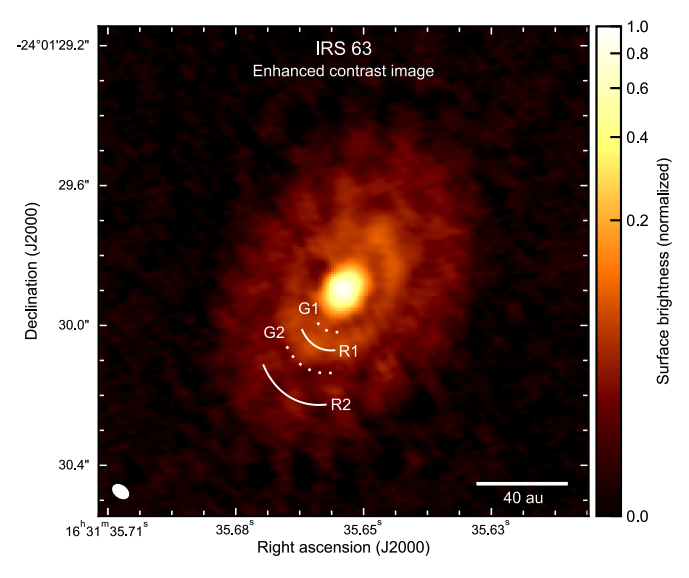
\includegraphics[width=\textwidth]{WRITEUP_AND_IMAGES/IMAGES/WRITEUP/NOTMINE/IRS63DomPlaceHolder.png}
        \captionof{figure}{Image of IRS 63 in dust continuum at \bsixNS, highlighting the substructure of the disk.  Image from \cite{Dom2020}. \note{ask for permission} \add{higher resolution image}}
        \label{fig: IRS63Dom2024}
    \end{minipage}
    \hfill 
    \begin{minipage}[t]{0.48\textwidth}
        \centering
        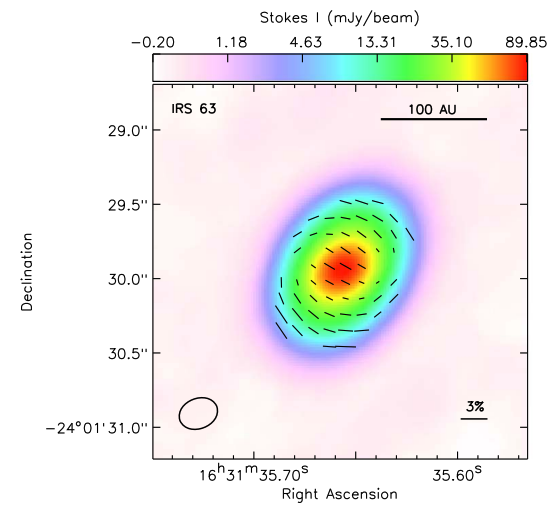
\includegraphics[width=\textwidth]{WRITEUP_AND_IMAGES/IMAGES/WRITEUP/NOTMINE/Sadavoy2019.png}
        \captionof{\SI image of IRS 63 at \bsixmmNS. Polarization vectors are shown as black lines and are scaled by polarization fraction. {\add{caption} Image from \cite{sadavoy_dust_2019}. \add{higher resolution image} \note{ask for permission}}
        \label{fig: IRS63Sadavoy2019}
    \end{minipage}

\end{figure*}
